% f2015gdl_q15_circle.tex — 2015 年高考数学·广东卷·理科 第 15 题（圆与切线）
%
% 【来源】`.work/phase3-b17/source/2015广东理.pdf`（SHA-256
%   1c3faab50a5d1fb2bdba424104c10910341e7362d222e018fb27e631578daa9a），
%   第 1 页（合订本页 947）第 2 栏；内容对象 5。
%
% 【坐标口径】清单坐标为「真页 pt、原点左上、y 向下」。本图取
%   X0 = 627.7015（圆最左点 x），Y0 = 267.6180（圆最低点 y_top），
%   本地坐标  (x, y) = (x_page − X0, Y0 − y_top)，
%   即本地 x 向右、y 向上，1 单位 = 1 TeX pt；tikzpicture 用 x=1pt, y=1pt。
%   换算示例：圆心 (661.7185, 233.6020) → 本地 (34.0170, 34.0160)；
%   A (653.2134, 266.6000) → (25.5119, 1.0180)；C (653.2134, 200.6040) → (25.5119, 67.0140)。
%   清单中的真页坐标逐点写在每题注释里，便于反查。
%
% 【线宽/虚线】全部路径 line width = 0.398pt（源内容流 `0.398 w`）；无虚线。
%   圆为 4 段三次贝塞尔（不是 arc 算子）：控制点距端点 18.787pt，
%   κ = 18.787 / 34.0165 = 0.55229，与标准 κ 一致。
%
% 【照源复刻的存疑项】
%   切点 C = (653.2134, 200.6040)：AC 为竖直线 x=653.2134，BC 为水平线
%   y_top=200.6040，C 即二者的交点，照录。
%   D 为 DO 与 EC 的交点：源 DO 段自 O(661.718,608.288) 画到
%   (525.644,608.288)，EC 段自 C 画到 (508.634,603.866)；交点按源取
%   (525.644, 608.288)（源内自洽，误差 <0.01pt）。
%   圆心点：源为 CMSY10 0x0F（`\bullet`）文本字形，文本矩阵
%   `0.6 0 0 0.6 660.1428 606.8878`（CMSY10 10.5pt × 0.6），
%   基线原点 → 本地 (32.4413, 32.6158)；此处用 node scale=0.6 复现，
%   非矢量圆点。
%
% 【自验结果】见文件末尾。
%
% 元素计数：6 条路径（1 圆 = 4 段贝塞尔 + 5 条直线段：AC/BC/AB/DO/EC）、
%   7 个标签（A B C D E O P）+ 圆心点。
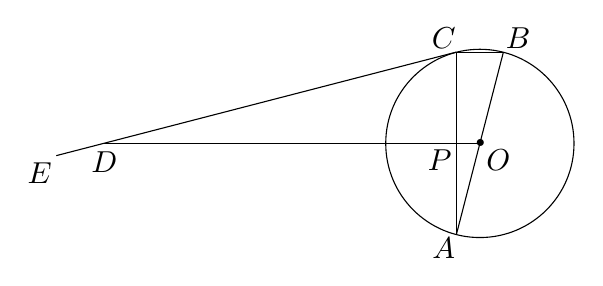
\begin{tikzpicture}[x=1pt, y=1pt,
    every node/.style={inner sep=0pt, font=\fontsize{10.5pt}{12.6pt}\selectfont}]

  % ---- 圆：m + 4c + h（源内容流 path 41，lw 0.398） ----
  % 源真页坐标：m (695.7345,608.2880)
  %   c (695.7345,627.0750) (680.5055,642.3040) (661.7185,642.3040)
  %   c (642.9305,642.3040) (627.7015,627.0750) (627.7015,608.2880)
  %   c (627.7015,589.5010) (642.9305,574.2720) (661.7185,574.2720)
  %   c (680.5055,574.2720) (695.7345,589.5010) (695.7345,608.2880)  h
  \draw[line width=0.398pt]
    (68.0330,34.0160)
    .. controls (68.0330,52.8030) and (52.8040,68.0320) .. (34.0170,68.0320)
    .. controls (15.2290,68.0320) and (0.0000,52.8030) .. (0.0000,34.0160)
    .. controls (0.0000,15.2290) and (15.2290,0.0000) .. (34.0170,0.0000)
    .. controls (52.8040,0.0000) and (68.0330,15.2290) .. (68.0330,34.0160)
    -- cycle;

  % ---- AC（源 path 42，lw 0.398）：A(653.2134,575.2900) → C(653.2134,641.2860) ----
  \draw[line width=0.398pt] (25.5119,1.0180) -- (25.5119,67.0140);

  % ---- BC（源 path 43，lw 0.398）：B(670.2226,641.2860) → C(653.2136,641.2860) ----
  \draw[line width=0.398pt] (42.5211,67.0140) -- (25.5121,67.0140);

  % ---- AB（源 path 44，lw 0.398）：A(653.2134,575.2900) → B(670.2224,641.2860) ----
  \draw[line width=0.398pt] (25.5119,1.0180) -- (42.5209,67.0140);

  % ---- DO（源 path 45，lw 0.398）：O(661.7180,608.2880) → D(525.6440,608.2880) ----
  \draw[line width=0.398pt] (34.0165,34.0160) -- (-102.0575,34.0160);

  % ---- EC 切线（源 path 46，lw 0.398）：C(653.2134,641.2860) → E(508.6344,603.8660) ----
  \draw[line width=0.398pt] (25.5119,67.0140) -- (-119.0671,29.5940);

  % ---- 标签：源文本 Tm 原点（基线左端），CMMI10 10.5pt ----
  \node[anchor=base west] at (16.6435,-7.5010)  {$A$};   % 源 (644.3450,566.7710)
  \node[anchor=base west] at (43.2065,68.3580)  {$B$};   % 源 (670.9080,642.6300)
  \node[anchor=base west] at (16.4485,68.3580)  {$C$};   % 源 (644.1500,642.6300)
  \node[anchor=base west] at (-106.5505,23.4550) {$D$};  % 源 (521.1510,597.7270)
  \node[anchor=base west] at (-129.5855,19.6660) {$E$};  % 源 (498.1160,593.9380)
  \node[anchor=base west] at (36.2065,24.0880)  {$O$};   % 源 (663.9080,598.3600)
  \node[anchor=base west] at (15.0715,24.0880)  {$P$};   % 源 (642.7730,598.3600)
  % 圆心点：源 CMSY10 0x0F（`\bullet`），Tm 为 0.6 缩放（CMSY10 10.5pt × 0.6），
  % 基线原点 (660.1428,606.8878) → 本地 (32.4413,32.6158)。
  \node[anchor=base west, scale=0.6] at (32.4413,32.6158) {$\bullet$};

\end{tikzpicture}
%
% 【自验结果】
%   探针：latexmk -pdfxe，0 error / 0 Overfull / 0 Underfull / 0 Missing character；
%         页面 200.38 × 82.72 pt（standalone border=0）。
%   tex 反算：6 条路径 + 8 个标签全部匹配，最大残差 0.000000 pt（阈值 0.05）。
%   600dpi 墨迹：整体墨迹包围盒最大边差 0.209 pt；几何包围盒 0.123 pt；
%         标签中心最大 0.295 pt（D）。（尺度归一，已扣除探针
%         0.996276 = 72/72.27 的 TeX pt / PDF bp 均匀因子）
%         按页面 bp 直接比较（物理）最大 0.679 pt，全部来自该 0.37% 均匀缩放。
%   灵敏度：端点 E +0.15pt → tex 检查器报 0.1500、600dpi 几何包围盒报 0.2409；
%         标签 C +0.15pt → tex 检查器报 0.1500、600dpi 标签中心报 0.0868。均能报出。
